\documentclass[12pt, twoside]{article}
\usepackage[letterpaper, margin=1in, headsep=0.2in]{geometry}
\setlength{\headheight}{0.6in}
%\usepackage[english]{babel}
\usepackage[utf8]{inputenc}
\usepackage{microtype}
\usepackage{amsmath}
\usepackage{amssymb}
%\usepackage{amsfonts}
\usepackage{siunitx} %units in math. eg 20\milli\meter
\usepackage{yhmath} % for arcs, overparenth command
\usepackage{tikz} %graphics
\usetikzlibrary{quotes, angles}
\usepackage{graphicx} %consider setting \graphicspath{{images/}}
\usepackage{parskip} %no paragraph indent
\usepackage{enumitem}
\usepackage{multicol}
\usepackage{venndiagram}

\usepackage{fancyhdr}
\pagestyle{fancy}
\fancyhf{}
\renewcommand{\headrulewidth}{0pt} % disable the underline of the header
\raggedbottom
\hfuzz=2mm %suppresses overfull box warnings

\usepackage{hyperref}

\fancyhead[LE]{\thepage}
\fancyhead[RO]{\thepage \\ Name: \hspace{4cm} \,\\}
\fancyhead[LO]{BECA / Dr. Huson / Geometry\\*  Unit 1: Segments, length, and area\\* 19 Sept 2022}

\begin{document}

\subsubsection*{1.8 Classwork: Area of rectangles, triangles, parallelograms}
\begin{enumerate}
\item Find the area of $\triangle ABC$,  $Area= \frac{1}{2}bh$. The altitude $h$ of the triangle is 3 centimeters and the base $AB=6$ cm.\\[0.5cm]
   \begin{tikzpicture}[scale=1]
     \draw [thick]
       (2,0)node[below]{$A$}--
       (8,0)node[below]{$B$}--
       (4,3)node[above]{$C$} --(2,0);
    \draw [dashed] (4,0)--(4,3);
    \draw (4,0)++(0.3,0)--++(0,0.3)--+(-0.3,0);
    \node at (4,1.2)[right]{$h=3$};
    \node at (5,0)[below]{$6$ cm};
  \end{tikzpicture} \vspace{1.0cm}

\item Find the area of $\triangle ABC$ shown below (not actual size) with $m\angle C=90^\circ$ and the lengths of the triangle's sides as $a=50$, $b=87$, and $c=100$. \\ \vspace{0.1cm}
      \begin{tikzpicture}[scale=1.4]
        \draw [thick]
        (0,0)node[left]{$A$}--
        (4,0)node[below right]{$C$}--
        (4,2.31)node[right]{$B$}--cycle;
        \draw (4,0)++(-0.3,0)--++(0,0.3)--+(0.3,0);
        \node at (2,0)[below]{$b=87$};
        \node at (4,1.2)[right]{$a=50$};
        \node at (1.8,1.4)[above]{$c=100$};
      \end{tikzpicture}
  \vspace{2.5cm}

\item Draw and label a triangle $\triangle ABC$ with base $\overline{AB}$ 8 centimeters long and altitude of 5 centimeters. (show the altitude as a dotted line, and make sure it is perpendicular to the base) 

\newpage

\item Given the rectangle $ABCD$, shown below, with $AB=11$ and $AD=5$. Find its area.
    \begin{flushright}
    \begin{tikzpicture}[scale=0.6]
      \draw [-, thick] (0,0)--(7,0)--(7,4)--(0,4)--cycle;
      \draw [fill] (0,0) circle [radius=0.05] node[left]{$A$};
      \draw [fill] (7,0) circle [radius=0.05] node[right]{$B$};
      \draw [fill] (7,4) circle [radius=0.05] node[right]{$C$};
      \draw [fill] (0,4) circle [radius=0.05] node[left]{$D$};
      \node at (-0.5, 2){5};
      \node at (3.5, -0.5){11};
    \end{tikzpicture}
    \end{flushright}

\item Find the area of the rectangle $MATH$ shown below, with $MA=4.7$ and $MH=1.9$.
    \begin{flushleft}
    \begin{tikzpicture}
      \draw [-, thick] (0,0)--(5,0)--(5,2)--(0,2)--cycle;
      \draw [fill] (0,0) circle [radius=0.05] node[left]{$M$};
      \draw [fill] (5,0) circle [radius=0.05] node[right]{$A$};
      \draw [fill] (5,2) circle [radius=0.05] node[right]{$T$};
      \draw [fill] (0,2) circle [radius=0.05] node[left]{$H$};
      \node at (-0.5, 1){1.9};
      \node at (2.5, -0.5){4.7};
    \end{tikzpicture}
    \end{flushleft}

\newpage

\item Find the combined area of the shape shown below, a rectangle and a square. The grid is in centimeters.
    \begin{flushleft}
      \begin{tikzpicture}[scale=1]
        \draw [help lines] (-4,-4) grid (5,3);
        %\draw [thick, ->] (-2.2,0) -- (10.4,0) node [below right] {$x$};
        %\draw [thick, ->] (0,-2.2)--(0,10.4) node [left] {$y$};
        %\draw (0,0) circle [radius=3] node[below]{$C$};
        %\draw [fill] (0,0) circle [radius=0.05];
        \draw [thick, -] (-3,-3)--(4,-3)--(4,0)--(-1,0)--(-1,2)--(-3,2)--cycle;
      \end{tikzpicture}
    \end{flushleft} \vspace{0.5cm} 

\item The compound shape shown below is composed of a square with side length 5 cm and a triangle with base 2 cm. Find the total area of the combined shape.
    \vspace{1cm} 
    \begin{flushleft}
    \begin{tikzpicture}
      \draw [-, thick] (0,0)--(7,0)--(5,5)--(0,5)--cycle;
      \draw [dashed] (5,0)--(5,5);
      %\draw [fill] (0,0) circle [radius=0.05] node[left]{$A$};
      %\draw [fill] (7,0) circle [radius=0.05] node[right]{$B$};
      %\draw [fill] (7,2) circle [radius=0.05] node[right]{$C$};
      %\draw [fill] (0,2) circle [radius=0.05] node[left]{$D$};
      \node at (6, -0.5){2};
      \node at (2.5, -0.5){5};
      \node at (-0.5, 2.5){5};
    \end{tikzpicture}
    \end{flushleft} \vspace{1cm}
\item Repeat the calculation for the figure above using the trapezoid area formula.

\item Find the area $A$ and perimeter $P$ of a square with sides of length 10 centimeters. \vspace{4cm}
    
  \item Find the area $A$ and perimeter $P$ of the shape shown below. The grid is in centimeters.
      \begin{flushleft}
        \begin{tikzpicture}[scale=1]
          \draw [help lines] (-4,-4) grid (5,3);
          %\draw [thick, ->] (-2.2,0) -- (10.4,0) node [below right] {$x$};
          %\draw [thick, ->] (0,-2.2)--(0,10.4) node [left] {$y$};
          %\draw (0,0) circle [radius=3] node[below]{$C$};
          %\draw [fill] (0,0) circle [radius=0.05];
          \draw [thick, -] (-3,-3)--(4,-3)--(4,2)--(2,2)--(2,0)--(-1,0)--(-1,2)--(-3,2)--cycle;
        \end{tikzpicture}
      \end{flushleft}
        
  \item The area of a square is 100 square centimeters. Find the length of the side of the square. \vspace{3cm}
      
  \item The perimeter of a square is 100 square centimeters. Find the length of the side of the square.
  
\newpage
\item On the grid below, accurately draw and label two adjacent squares, one with a side length of 4 cm, the other with a side length of 3 cm. The grid is in centimeters.\\*[5pt]
  Find the area $A$ and perimeter $P$ of combined shape.
  \begin{flushleft}
    \begin{tikzpicture}[scale=1]
      \draw [help lines] (-4,-3) grid (5,3);
      %\draw [thick, ->] (-2.2,0) -- (10.4,0) node [below right] {$x$};
      %\draw [thick, ->] (0,-2.2)--(0,10.4) node [left] {$y$};
      %\draw (0,0) circle [radius=3] node[below]{$C$};
      %\draw [fill] (0,0) circle [radius=0.05];
      %\draw [thick, -] (-3,-3)--(4,-3);
    \end{tikzpicture}
  \end{flushleft}

\item The rectangle $MATH$ has an area of 102, with length $MA=12$. Find the width of the rectangle $AT$.
\begin{flushleft}
\begin{tikzpicture}
  \draw [-, thick] (0,0)--(4,0)--(4,3)--(0,3)--cycle;
  \draw [fill] (0,0) circle [radius=0.05] node[left]{$M$};
  \draw [fill] (4,0) circle [radius=0.05] node[right]{$A$};
  \draw [fill] (4,3) circle [radius=0.05] node[right]{$T$};
  \draw [fill] (0,3) circle [radius=0.05] node[left]{$H$};
  \node at (4.5, 1.5){?};
  \node at (2, -0.5){12};
\end{tikzpicture}
\end{flushleft} \vspace{1cm} 

\item One side of the $\triangle ABC$ has a length $AB=8$. The triangle's area is 44. Find the length of the altitude $h$ of the triangle to vertex $C$ and perpendicular to side $\overline{AB}$.\\[0.5cm]
  \begin{tikzpicture}[scale=1, rotate=-40]
    \draw [thick]
      (2,0)node[below]{$A$}--
      (8,0)node[below]{$B$}--
      (5,3)node[above]{$C$} --(2,0);
    \draw [dashed] (5,0)--(5,3);
    \draw (5,0)++(0.3,0)--++(0,0.3)--+(-0.3,0);
    \node at (5,1)[right]{$h=?$};
    \node at (5,0)[below left]{$8$};
  \end{tikzpicture}


\item Find the area of $\triangle ABC$. The altitude $h$ of the triangle is $8$ centimeters and the base $AB=10 \frac{1}{2}$ cm. (diagram not to scale) \\[0.5cm]
\begin{tikzpicture}[scale=1.]
  \draw [thick]
    (2,0)node[below]{$A$}--
    (8,0)node[below]{$B$}--
    (4,3)node[above]{$C$} --(2,0);
 \draw [dashed] (4,0)--(4,3);
 \draw (4,0)++(0.3,0)--++(0,0.3)--+(-0.3,0);
 \node at (4,1.2)[right]{$h=8$};
 \node at (5,0)[below]{$10 \frac{1}{2}$ cm};
\end{tikzpicture} 

\item The compound shape shown below is composed of a rectangle 3 inches by 7 inches, and a triangle with base 2 inches. Find the total area of the combined shape.
    \vspace{0.5cm} 
    \begin{flushleft}
    \begin{tikzpicture}
      \draw [-, thick] (0,0)--(7,0)--(5,3)--(0,3)--cycle;
      \draw [dashed] (5,0)--(5,3);
      %\draw [fill] (0,0) circle [radius=0.05] node[left]{$A$};
      %\draw [fill] (7,0) circle [radius=0.05] node[right]{$B$};
      %\draw [fill] (7,2) circle [radius=0.05] node[right]{$C$};
      %\draw [fill] (0,2) circle [radius=0.05] node[left]{$D$};
      \node at (6, -0.5){2};
      \node at (2.5, -0.5){7};
      \node at (-0.5, 1.5){3};
    \end{tikzpicture}
    \end{flushleft}
        
\item The area of a square is 36 square centimeters. Find the length of the side of the square. \vspace{3cm}

\item One side of the $\triangle ABC$ has a length $AB=12$. The triangle's area is 60. Find the length of the altitude $h$ of the triangle to vertex $C$ and perpendicular to side $\overline{AB}$.\\
\begin{tikzpicture}[scale=0.9, rotate=30]
  \draw [thick]
    (2,0)node[below]{$A$}--
    (8,0)node[below]{$B$}--
    (5,3)node[above]{$C$} --(2,0);
  \draw [dashed] (5,0)--(5,3);
  \draw (5,0)++(0.3,0)--++(0,0.3)--+(-0.3,0);
  \node at (5.2,1.5)[right]{$h=?$};
  \node at (5,-0.5)[below left]{$12$};
\end{tikzpicture}

\item Find the area of $\triangle ABC$ shown below (not actual size) with $m\angle C=90^\circ$ and the lengths of the triangle's sides as $a=3$, $b=4$, and $c=5$. 
\begin{flushright}
\begin{tikzpicture}[scale=1.4]
  \draw [thick]
  (0,0)node[left]{$A$}--
  (4,0)node[below right]{$C$}--
  (4,2.31)node[right]{$B$}--cycle;
  \draw (4,0)++(-0.3,0)--++(0,0.3)--+(0.3,0);
  \node at (2,0)[below]{$b=4$};
  \node at (4,1.2)[right]{$a=3$};
  \node at (1.8,1.4)[above]{$c=5$};
\end{tikzpicture}
\end{flushright}
\vspace{1cm}

\item Find the area and perimeter of the shape shown below. Mark the missing side lengths first. All angles are $90^\circ$.\hfill \emph{(not drawn to scale)}
\begin{flushleft}
\begin{tikzpicture}[rotate=-90, scale=1.2]
\draw [-, thick] (2,0)--(4.5,0)--(4.5,2.5)--(3,2.5)--(3,5)--(2,5)--cycle;
%\draw [fill] (0,0) circle [radius=0.05] node[left]{$A$};
%\draw [fill] (7,0) circle [radius=0.05] node[right]{$B$};
%\draw [fill] (7,2) circle [radius=0.05] node[right]{$C$};
%\draw [fill] (0,2) circle [radius=0.05] node[left]{$D$};
\node at (5.1, 1.2){6};
\node at (4, 2.8){5};
\node at (3.5, -0.5){7};
\node at (1.4, 2.5){11};
\end{tikzpicture}
\end{flushleft} \vspace{1cm}


\end{enumerate}
\end{document}